%\documentclass[a4paper,11pt,fleqn]{report}
%\documentclass[a4paper,11pt,twoside]{report}
\documentclass[a4paper,12pt,]{report}
\usepackage[utf8x]{inputenc}
\usepackage[T1]{fontenc}
\usepackage[german, ngerman]{babel}
\usepackage{longtable}
\usepackage[BCOR0.5cm]{typearea} %deaktivate
\usepackage{tabularx}
\usepackage{latexsym}
\usepackage{amsmath,mathptmx} %  Times-Schriftart
\usepackage{graphicx,float}
\usepackage{helvet}
\usepackage{fancyheadings}
\pagestyle{fancy}
\usepackage{geometry}
\usepackage{microtype}
\geometry{a4paper, top=30mm, left=25mm, right=25mm, bottom=0mm,
headsep=10mm, footskip=10mm}
%\usepackage{amsfonts}
\usepackage{listings}
\setlength{\headwidth}{16cm}
\setlength{\textwidth}{16cm}
\setlength{\leftmargin}{-1cm}

\renewcommand{\chaptermark}[1]%
                  {\markboth{#1}{}}

\renewcommand{\sectionmark}[1]%
               {\markright{\thesection\ #1}}
\lhead[\fancyplain{}{\bfseries\thepage}]%
     {\fancyplain{}{\bfseries\rightmark}}
\rhead[\fancyplain{}{\bfseries\leftmark}]%
      {\fancyplain{}{\bfseries\thepage}}
\cfoot{}

\setlength{\parindent}{0pt} %kein einzug nach Absatz

\renewcommand{\baselinestretch}{1.2} 
\usepackage{lscape} 
\setlength{\textheight}{24.5cm}

%\usepackage[hang, rm, bf]{caption}
\usepackage[font=small,format=plain,labelfont=bf,up,textfont=rm,rm]{caption}
\clubpenalty = 10000 
\widowpenalty = 10000 
\displaywidowpenalty = 10000
\begin{document}

\thispagestyle{empty}


\begin{figure}[t]
\vspace{-3cm}
\begin{minipage}[t]{3cm}
\vspace{-2cm}

\includegraphics[width=6cm]{Deckblatt/Wortmarke_RUB.jpg}
\end{minipage}
\hfill
\begin{minipage}[t]{3cm}

\includegraphics[width=3cm]{Deckblatt/Label_RUB.jpg}
\end{minipage}
\vspace{3cm}
\end{figure}


\renewcommand{\rmdefault}{phv}
\begin{center}


	{\Huge \bf P R O J E K T A R B E I T}
	
	\vspace{0.5cm}
	
	{\Large
	zum Thema:\\
	\vspace{0.5cm}
	Entwicklung eines Server-Client Systems zur Darstellung PDF-basierter Präsentationen\\
	\vspace{0.5cm}
	von\\
	\vspace{0.5cm}
	{\LARGE \bf
	René Beckmann\\
	Sascha Brexeler\\
	Diana Castano\\
	Tim Hebbeler\\
	Jens Helge Micke\\
	}
	\vspace{0.5cm}
	}
\end{center}

\begin{table}[h!]
\begin{tabular}{p{0.5\textwidth}p{0.5\textwidth}}
Betreuender Dozent & Dr. Wolfgang Theimer\\
&\\
&\\
&\\
&\\
&\\
Beginn: & 13.04.2016\\
&\\
Abgabe: & 20.07.2016\\
\end{tabular}
\end{table}

\renewcommand{\rmdefault}{ptm}

\pagenumbering{Roman}
\setcounter{secnumdepth}{3}
\setcounter{tocdepth}{2}
{\parskip=4mm \tableofcontents}
\newpage
\listoffigures
\newpage
\pagenumbering{arabic}

%\include{Erklaerung/Erklaerung}

\setcounter{page}{1}

\chapter{Einleitung}
\thispagestyle{fancy}


% !TeX encoding = UTF-8
\chapter{Latex Beispiel}
\thispagestyle{fancy}
\label{LatexBeispiel}
Über das chapter Steuerzeichen werden Überschriften generiert.\\
Über das label Steuerzeichen können Referenzmarken geschaffen werden die über \mbox{(siehe Kap. \ref{LatexBeispiel}  S. \pageref{LatexBeispiel})} referenziert werden können.
Dazu muss jedoch das Dokument zwei Mal berechnet werden.
\section{Unter einem Chapter kommt eine Section}
Eine Section wird numeriert und taucht im Inhaltsverzeichnis auf.
\subsection{Unter einer Section eine Subsection}
Eine SubSection wird numeriert und taucht im Inhaltsverzeichnis auf.
\subsubsection{Unter einer Subsection eine SubSubSection}
Eine SubSubSection wird numeriert und taucht in diesem Falle nicht im Inhaltsverzeichnis auf.
\paragraph{Ein Paragraph}$\;$\\
Ein Paragraph erhält keine Nummerierung, dafür eine fette Überschrift und wird nicht im Inhaltsverzeichnis aufgezählt.
\\ %Leerzeile
Fußnote\footnote{\mbox{Innenwiderstand $20m\Omega$ $\rightarrow$ $\frac{1,35V-0,85V}{20m\Omega}=25A$ Ladestrom}} mit grenzeneinhaltender Mathematik.
Einfache Elemente kann man auch so: $V_{high}$ einbinden.
oder als numerierte Equation
\begin{equation} \label{eq:Tiefpass24}
|A|=\sqrt{\frac{(1-\omega^{2}R_{1}C_{1}R_{2}C_{2})^{2}+(\omega(R_{1}C_{1}+R_{2}C_{2}))^{2}}{\left( (1-\omega^{2}R_{1}C_{1}R_{2}C_{2})^{2}+(\omega(R_{1}C_{1}+R_{2}C_{2}))^{2}\right)^{2}}}
\end{equation}

Zitiere Eric C. Darcy\cite{Darcy} aus der Bibliothek.

\begin{figure}[ht!]
\centering
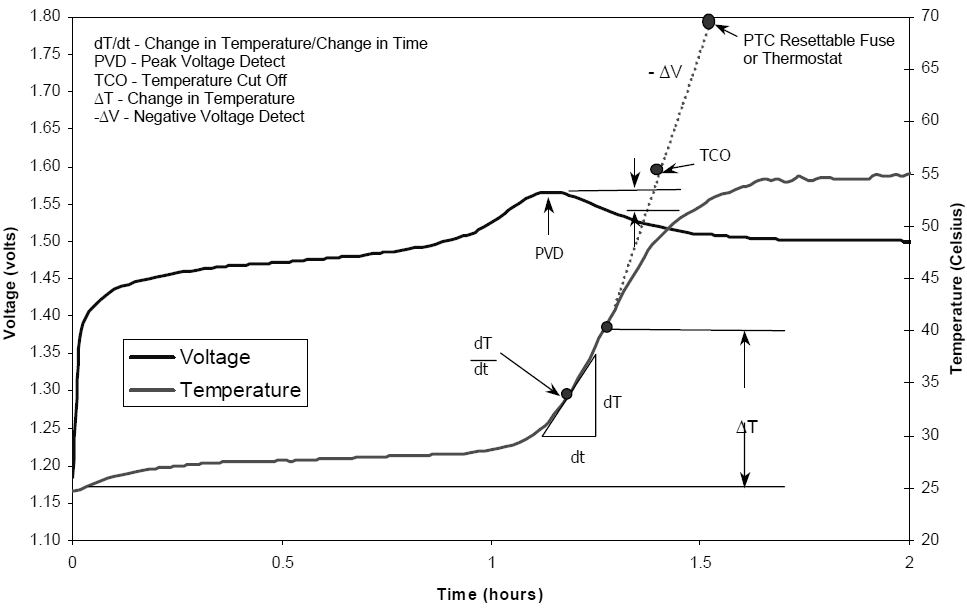
\includegraphics[angle=0,width=14cm]{LatexBeispiel/Bilder/Ladeschlussbw.png}
\caption{Ladeschlusserkennungen, Harding Battery Handbook\cite{Harding}}
\label{Ladeschluss}
\end{figure}

\newpage
So kann Code eingefügt werden.
\begin{lstlisting}[frame=single,breaklines=true,basicstyle=\tiny,language=C,label={PWMStart},caption={Kommentierter Start der PWM}]
/*! \brief Starts the PWM
 * 
 * To make sure that the PWM behaves correctly after a Compare Bit Change the PWM is started and reset with a software trigger.
 */
static void vStartPwm( void )
{
	tc_start( &AVR32_TC0, PWM_CHANNEL );
	tc_software_trigger( &AVR32_TC0, PWM_CHANNEL );
}
\end{lstlisting}


%\addcontentsline{toc}{chapter}{Danksagung}
%\include{Danksagung/Danksagung}

\addcontentsline{toc}{chapter}{Literaturverzeichnis}
\bibliography{Literaturverzeichnis/biblio}
\bibliographystyle{Literaturverzeichnis/unsrtdin_pi}

\end{document}
